\documentclass{ximera}

\input{../../preamble.tex}

\title{Examples of Injective Linear Transformations}

\begin{document}
\begin{abstract}
  We consider examples of injective functions, and examples that are not injective.
\end{abstract}
\maketitle

It is perhaps most instructive to examine a linear transformation that is not injective first.

\begin{example}[Not injective]

Consider the linear transformation
\[
\ltdefn{T}{\complex{5}}{\complex{5}},\quad
\lteval{T}{\colvector{x_1\\x_2\\x_3\\x_4\\x_5}}=
\colvector{-2 x_1 + 3 x_2 + 3 x_3 - 6 x_4 + 3 x_5\\
-16 x_1 + 9 x_2 + 12 x_3 - 28 x_4 + 28 x_5\\
-19 x_1 + 7 x_2 + 14 x_3 - 32 x_4 + 37 x_5\\
-21 x_1 + 9 x_2 + 15 x_3 - 35 x_4 + 39 x_5\\
-9 x_1 + 5 x_2 + 7 x_3 - 16 x_4 + 16 x_5}
\]

Notice that for
\begin{align*}
\vect{x}&=\colvector{1\\3\\-1\\2\\4}&
\vect{y}&=\colvector{4\\7\\0\\5\\7}
\end{align*}
so we have
\begin{align*}
\lteval{T}{\colvector{1\\3\\-1\\2\\4}}&=\colvector{4\\55\\72\\77\\31}&
\lteval{T}{\colvector{4\\7\\0\\5\\7}}&=\colvector{4\\55\\72\\77\\31}
\end{align*}

So we have two vectors from the domain, $\vect{x}\neq\vect{y}$, yet $\lteval{T}{\vect{x}}=\lteval{T}{\vect{y}}$, in violation of \ref{definition:ILT}.  This is another example where you should not concern yourself with how $\vect{x}$ and $\vect{y}$ were selected, as this will be explained shortly.  However, do understand \textit{why} these two vectors provide enough evidence to conclude that $T$ is not injective.

\end{example}

Here is a cartoon of a non-injective linear transformation.  Notice that the central feature of this cartoon is that $\lteval{T}{\vect{u}}=\vect{v}=\lteval{T}{\vect{w}}$.  Even though this happens again with some unnamed vectors, it only takes one occurrence to destroy the possibility of injectivity.  Note also that the two vectors displayed in the bottom of $V$ have no bearing, either way, on the injectivity of $T$.
\begin{image}
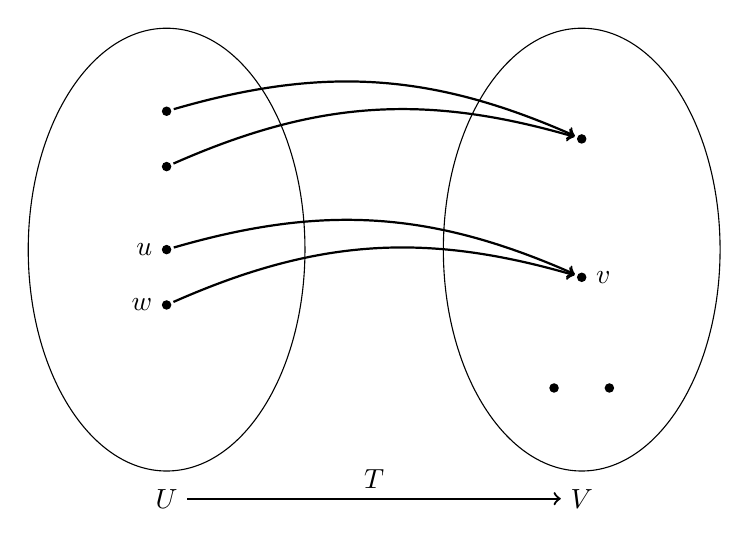
\begin{tikzpicture}
\tikzset{ltvect/.style={shape=circle, minimum size=0.30em, inner sep=0pt, draw, fill=black}}
\tikzset{ltedge/.style={->, bend left=20, thick, shorten <=0.1em, shorten >=0.1em}}
<!--  base generic picture -->
\draw ( 5em, 8em) circle [x radius=5em, y radius=8em, thick];
\draw (20em, 8em) circle [x radius=5em, y radius=8em, thick];
\node (U) at ( 5em, -1em) {$U$};
\node (V) at (20em, -1em) {$V$};
\draw[->, thick, draw] (U) to node[auto] {$T$} (V);
<!--  inputs -->
\node (u1) [ltvect]                         at (5em, 13em) {};
\node (u2) [ltvect]                         at (5em, 11em) {};
\node (u)  [ltvect, label=left:$\vect{u}$]  at (5em,  8em) {};
\node (w)  [ltvect, label=left:$\vect{w}$]  at (5em,  6em) {};
<!--  outputs -->
\node (v1) [ltvect]                         at (20em, 12em) {};
\node (v)  [ltvect, label=right:$\vect{v}$] at (20em,  7em) {};
\node (v2) [ltvect]                         at (19em,  3em) {};
\node (v3) [ltvect]                         at (21em,  3em) {};
<!--  associations -->
\draw[ltedge] (u1) to (v1);
\draw[ltedge] (u2) to (v1);
\draw[ltedge] (u)  to (v);
\draw[ltedge] (w)  to (v);
\end{tikzpicture}
\end{image}

To show that a linear transformation is not injective, it is enough to find a single pair of inputs that get sent to the identical output.  However, to show that a linear transformation is injective we must establish that this coincidence of outputs \textit{never} occurs.  Here is an example that shows how to establish this.

\begin{example}[Injective]

Consider the linear transformation
\[
\ltdefn{R}{\complex{5}}{\complex{5}},\quad
\lteval{R}{\colvector{x_1\\x_2\\x_3\\x_4\\x_5}}=
\colvector{-65 x_1 + 128 x_2 + 10 x_3 - 262 x_4 + 40 x_5\\
36 x_1 - 73 x_2 - x_3 + 151 x_4 - 16 x_5\\
-44 x_1 + 88 x_2 + 5 x_3 - 180 x_4 + 24 x_5\\
34 x_1 - 68 x_2 - 3 x_3 + 140 x_4 - 18 x_5\\
12 x_1 - 24 x_2 - x_3 + 49 x_4 - 5 x_5}
\]

To establish this is injective we must begin with the assumption that $\lteval{R}{\vect{x}}=\lteval{R}{\vect{y}}$ and somehow arrive at the conclusion that $\vect{x}=\vect{y}$.  Here we go,
\begin{align*}
\colvector{0\\0\\0\\0\\0}
&=\lteval{R}{\vect{x}}-\lteval{R}{\vect{y}}\\
&=\lteval{R}{\colvector{x_1\\x_2\\x_3\\x_4\\x_5}}-\lteval{R}{\colvector{y_1\\y_2\\y_3\\y_4\\y_5}}\\
&=
\colvector{-65 x_1 + 128 x_2 + 10 x_3 - 262 x_4 + 40 x_5\\
36 x_1 - 73 x_2 - x_3 + 151 x_4 - 16 x_5\\
-44 x_1 + 88 x_2 + 5 x_3 - 180 x_4 + 24 x_5\\
34 x_1 - 68 x_2 - 3 x_3 + 140 x_4 - 18 x_5\\
12 x_1 - 24 x_2 - x_3 + 49 x_4 - 5 x_5}\\
&\quad\quad-
\colvector{-65 y_1 + 128 y_2 + 10 y_3 - 262 y_4 + 40 y_5\\
36 y_1 - 73 y_2 - y_3 + 151 y_4 - 16 y_5\\
-44 y_1 + 88 y_2 + 5 y_3 - 180 y_4 + 24 y_5\\
34 y_1 - 68 y_2 - 3 y_3 + 140 y_4 - 18 y_5\\
12 y_1 - 24 y_2 - y_3 + 49 y_4 - 5 y_5}\\
&=
\colvector{-65 (x_1-y_1) + 128 (x_2-y_2) + 10 (x_3-y_3) - 262 (x_4-y_4) + 40 (x_5-y_5)\\
36 (x_1-y_1) - 73 (x_2-y_2) - (x_3-y_3) + 151 (x_4-y_4) - 16 (x_5-y_5)\\
-44 (x_1-y_1) + 88 (x_2-y_2) + 5 (x_3-y_3) - 180 (x_4-y_4) + 24 (x_5-y_5)\\
34 (x_1-y_1) - 68 (x_2-y_2) - 3 (x_3-y_3) + 140 (x_4-y_4) - 18 (x_5-y_5)\\
12 (x_1-y_1) - 24 (x_2-y_2) - (x_3-y_3) + 49 (x_4-y_4) - 5 (x_5-y_5)}\\
&=
\begin{bmatrix}
-65&128&10&-262&40\\
36&-73&-1&151&-16\\
-44&88&5&-180&24\\
34&-68&-3&140&-18\\
12&-24&-1&49&-5
\end{bmatrix}
\colvector{x_1-y_1\\x_2-y_2\\x_3-y_3\\x_4-y_4\\x_5-y_5}
\end{align*}


Now we recognize that we have a homogeneous system of 5 equations in 5 variables (the terms $x_i-y_i$ are the variables), so we row-reduce the coefficient matrix to
\[
\begin{bmatrix}
\leading{1}&0&0&0&0\\
0&\leading{1}&0&0&0\\
0&0&\leading{1}&0&0\\
0&0&0&\leading{1}&0\\
0&0&0&0&\leading{1}
\end{bmatrix}
\]




So the only solution is the trivial solution
\begin{align*}
x_1-y_1&=0&x_2-y_2&=0&x_3-y_3&=0&x_4-y_4&=0&x_5-y_5&=0
\end{align*}
and we conclude that indeed $\vect{x}=\vect{y}$.  By \ref{definition:ILT}, $T$ is injective.

\end{example}

Here is the cartoon for an injective linear transformation.  It is meant to suggest that we never have two inputs associated with a single output.  Again, the two lonely vectors at the bottom of $V$ have no bearing either way on the injectivity of $T$.
\begin{image}
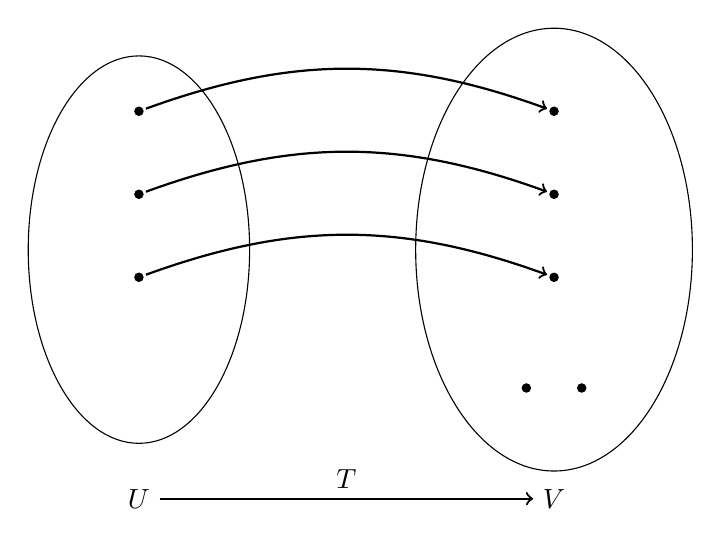
\begin{tikzpicture}
\tikzset{ltvect/.style={shape=circle, minimum size=0.30em, inner sep=0pt, draw, fill=black}}
\tikzset{ltedge/.style={->, bend left=20, thick, shorten <=0.1em, shorten >=0.1em}}
<!--  base generic picture -->
\draw ( 5em, 8em) circle [x radius=4em, y radius=7em, thick];
\draw (20em, 8em) circle [x radius=5em, y radius=8em, thick];
\node (U) at ( 5em, -1em) {$U$};
\node (V) at (20em, -1em) {$V$};
\draw[->, thick, draw] (U) to node[auto] {$T$} (V);
<!--  inputs -->
\node (u1) [ltvect] at (5em, 13em) {};
\node (u2) [ltvect] at (5em, 10em) {};
\node (u3) [ltvect] at (5em,  7em) {};
<!--  outputs -->
\node (v1) [ltvect] at (20em, 13em) {};
\node (v2) [ltvect] at (20em, 10em) {};
\node (v3) [ltvect] at (20em,  7em) {};
\node (v4) [ltvect] at (19em,  3em) {};
\node (v5) [ltvect] at (21em,  3em) {};
<!--  associations -->
\draw[ltedge] (u1) to (v1);
\draw[ltedge] (u2) to (v2);
\draw[ltedge] (u3) to (v3);
\end{tikzpicture}
\end{image}

Let us now examine an example between abstract vector spaces.

\begin{example}

Consider the linear transformation
\[
\ltdefn{T}{P_3}{M_{22}},\quad\lteval{T}{a+bx+cx^2+dx^3}=
\begin{bmatrix}
a+b & a-2c\\
d & b-d
\end{bmatrix}
\]

Suppose that two polynomial inputs yield the same output matrix,
\[
\lteval{T}{a_1+b_1x+c_1x^2+d_1x^3}=\lteval{T}{a_2+b_2x+c_2x^2+d_2x^3}
\]

Then
\begin{align*}
\zeromatrix
&=\begin{bmatrix}
0&0\\0&0
\end{bmatrix}\\
&=\lteval{T}{a_1+b_1x+c_1x^2+d_1x^3}-\lteval{T}{a_2+b_2x+c_2x^2+d_2x^3}&&\text{Hypothesis}\\
&=\lteval{T}{(a_1+b_1x+c_1x^2+d_1x^3)-(a_2+b_2x+c_2x^2+d_2x^3)}&&\ref{definition:LT}\\
&=\lteval{T}{(a_1-a_2)+(b_1-b_2)x+(c_1-c_2)x^2+(d_1-d_2)x^3}&&\text{Operations in $P_3$}\\
&=
\begin{bmatrix}
(a_1-a_2)+(b_1-b_2) & (a_1-a_2)-2(c_1-c_2)\\
(d_1-d_2) & (b_1-b_2)-(d_1-d_2)
\end{bmatrix}&&\text{Definition of $T$}
\end{align*}



This single matrix equality translates to the homogeneous system of equations in the variables $a_i-b_i$,
\begin{align*}
(a_1-a_2)+(b_1-b_2)&=0\\
(a_1-a_2)-2(c_1-c_2)&=0\\
(d_1-d_2)&=0\\
(b_1-b_2)-(d_1-d_2)&=0
\end{align*}




This system of equations can be rewritten as the matrix equation
\[
\begin{bmatrix}
1&1&0&0\\1&0&-2&0\\0&0&0&1\\0&1&0&-1
\end{bmatrix}
\colvector{(a_1-a_2)\\(b_1-b_2)\\(c_1-c_2)\\(d_1-d_2)}=\colvector{0\\0\\0\\0}
\]




Since the coefficient matrix is nonsingular (check this) the only solution is trivial, i.e.
\begin{align*}
a_1-a_2&=0&b_1-b_2&=0&c_1-c_2&=0&d_1-d_2&=0
\end{align*}
so that
\begin{align*}
a_1&=a_2&b_1&=b_2&c_1&=c_2&d_1&=d_2
\end{align*}
so the two inputs must be equal polynomials.  Therefore,
\begin{multipleChoice}
\choice[correct]{$T$ is injective.}
\choice{$T$ is not injective.}
\end{multipleChoice}

\end{example}

\end{document}
